\setauthor{\firstauthor}

\section{Technologie Stack}
\begin{figure}[H]
    \centering
    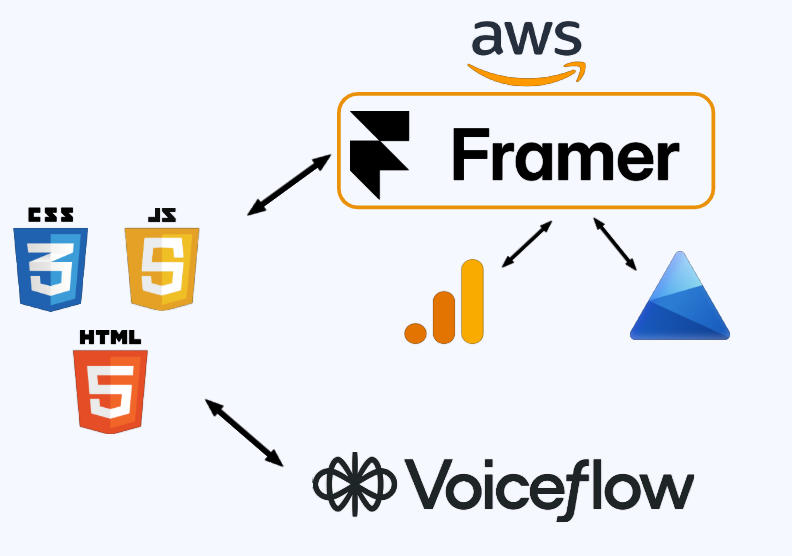
\includegraphics[scale=0.5]{pics/tech-stack.png}
    \caption{Technologie Stack}
    \label{fig:concept:tech-stack}
\end{figure}

Für die Umsetzung der beiden Funnel-Varianten wurde ein moderner und 
skalierbarer Tech-Stack gewählt, der sowohl eine effiziente Entwicklung als auch 
eine tiefgründige Analyse des Nutzerverhaltens ermöglicht. Die Frontend-Basis der 
Website besteht aus den Standard-Webtechnologien \textit{HTML}, \textit{CSS} und \textit{JavaScript}. Diese 
bilden die Grundlage für die Struktur, das Design und die Interaktivität der 
Benutzeroberfläche und ermöglichen eine plattformunabhängige Nutzung auf 
unterschiedlichen Endgeräten.

Als zentrales Tool für die Entwicklung und das UI-Design wird \textit{Framer} 
eingesetzt. \textit{Framer} kombiniert visuelles Design mit funktionaler Umsetzung 
und erlaubt die Erstellung interaktiver, produktionsreifer Websites. 
Dadurch können Designentscheidungen direkt 
umgesetzt und optimiert werden, insbesondere im Hinblick auf User Experience 
und Conversion-Optimierung.

Das Hosting der Websites erfolgt über AWS (Amazon Web Services), 
das in \textit{Framer} integriert ist und eine unkomplizierte Veröffentlichung 
sowie Verwaltung der Websites ermöglicht. Durch die Nutzung 
von \textit{Amazon Web Services} wird eine hohe Verfügbarkeit
und eine stabile Performance gewährleistet.

Zur Analyse des Nutzerverhaltens und zur Auswertung der Funnel-Performance 
werden zwei Tracking-Tools eingesetzt.
Zum einen wird \textit{Google Analytics} verwendet, um umfassende Einblicke in das 
Nutzerverhalten zu erhalten.
Zum anderen wird \textit{Microsoft Clarity} eingesetzt, um detaillierte Informationen 
und Screencasts von Nutzerinteraktionen zu sammeln.
Die eingesetzten Tools ermöglichen die Erfassung von Kennzahlen wie Seitenaufrufen,
Verweildauer, Absprungraten sowie Conversion-Raten. Auf dieser Grundlage können 
Unterschiede zwischen den beiden
Funnel-Varianten objektiv bewertet werden.

Für die Umsetzung des dialogbasierten Chatbots wird \textit{Voiceflow} verwendet. 
\textit{Voiceflow} ist eine Plattform zur Entwicklung von Chatbots, 
die es ermöglicht, strukturierte Dialogflüsse zu definieren und in 
bestehende Webanwendungen zu integrieren. Der Chatbot übernimmt dabei die Funktion 
der Informationsvermittlung und Nutzerführung, indem er individuell auf Eingaben 
reagiert und den Entscheidungsprozess interaktiv gestaltet.

Durch die Kombination dieser Technologien entsteht ein umfassender
Tech-Stack, der sowohl die Entwicklung zweier unterschiedlicher Funnel-Ansätze 
als auch deren Analyse im Rahmen dieser Arbeit ermöglicht.

\section{Voiceflow}

\section{Alternativen zu Voiceflow}

\setauthor{\firstauthor}
\section{Framer}
Framer ist ein No-Code-Tool zur Erstellung und zum Hosting interaktiver Websites.
Es ermöglicht die effiziente Entwicklung von interaktiven und responsiven Benutzeroberflächen.

Eine weitere Funktion von Framer ist die Möglichkeit, dass mehrere
Personen gleichzeitig an einer Website arbeiten können, was 
die Zusammenarbeit innerhalb eines Teams erleichtert.

Über die \textit{Custom-Code}-Funktion von Framer ist es möglich,
eigenen Code in die Website zu integrieren, um zusätzliche Funktionen, 
wie etwa die Einbindung eines Chatbots oder die Erfassung von Nutzerdaten, zu 
realisieren.

\setauthor{\firstauthor}
\subsection{Hosting mit Framer}
Framer bietet die Möglichkeit, Websites direkt über die Plattform zu hosten.
Das interne Hosting erfolgt über Server von AWS (Amazon Web Services), 
wobei die Website unter einer Subdomain der Form \textit{framer.app} bereitgestellt wird.
Alternativ besteht die Möglichkeit, die Website auf einem eigenen Server zu betreiben.

Durch den integrierten Hosting-Service können Änderungen innerhalb weniger Sekunden
veröffentlicht werden, was den Entwicklungsprozess deutlich beschleunigt.
Zudem wird jede veröffentlichte Änderung automatisch versioniert,
wodurch frühere Zustände bei Bedarf einfach wiederhergestellt werden können.

Darüber hinaus ist das Hosting über Framer bis zu einer Bandbreite von
1 Gigabyte pro Monat kostenlos,
während beim Betrieb auf einem eigenen Server zusätzliche Kosten entstehen.

\setauthor{\firstauthor}
\section{Alternativen zu Framer}
Mögliche Alternativen zu Framer sind Dienste wie Webflow oder Wix,
die ebenfalls die Erstellung interaktiver Websites ermöglichen.
Diese Plattformen bieten vergleichbare Funktionen, 
wie beispielsweise die Integration von eigenem Code sowie Hosting-Lösungen.

Dennoch weist Framer in einigen Bereichen Vorteile gegenüber den genannten
Alternativen auf. Dazu zählen unter anderem:
\begin{itemize}
    \item Die Möglichkeit, Änderungen an der Website innerhalb 
    weniger Sekunden zu veröffentlichen, was den Entwicklungsprozess 
    beschleunigt.
    \item Eine automatische Versionierung veröffentlichter Änderungen, 
    die ein einfaches Zurücksetzen auf frühere Versionen ermöglicht.
    \item Eine kostenlose Hosting-Option mit einer Bandbreite von 
    bis zu 1 Gigabyte pro Monat, wodurch Kosten reduziert werden.
    \item Eine gute Integration mit externen Tools, wie beispielsweise 
    Voiceflow, was die Entwicklung zusätzlich unterstützt.
    \item Flexible Gestaltungsmöglichkeiten durch die Einbindung 
    eigener CSS-Styles.
\end{itemize}

\section{Quarkus}

\section{Datenbank}

\section{D3.js}

\section{Nutzerdatenerfassung}

%\ mehr für Funnel
